\documentclass[xcolor=svgnames,14pt]{beamer}
\usepackage[utf8]{inputenc}
\usepackage{color}
\usepackage{bbding,verbatim,graphicx,tikz,listings,comment}

\usetikzlibrary{calc,trees,positioning,arrows,chains,shapes.geometric,%
    decorations.pathreplacing,decorations.pathmorphing,shapes,%
    matrix,shapes.symbols, decorations.markings}
\usetheme{Parasim}

\definecolor{javared}{rgb}{0.6,0,0} % for strings
\definecolor{javagreen}{rgb}{0.25,0.5,0.35} % comments
\definecolor{javapurple}{rgb}{0.5,0,0.35} % keywords
\definecolor{javadocblue}{rgb}{0.25,0.35,0.75} % javadoc

\lstset{
	language=Java,
	basicstyle=\scriptsize\ttfamily,
	keywordstyle=\color{javapurple}\bfseries,
	stringstyle=\color{javared},
	commentstyle=\color{javagreen},
	morecomment=[s][\color{javadocblue}]{/**}{*/},
	numbers=left,
	frame=leftline,
	numberstyle=\tiny\color{black},
	stepnumber=1,
	tabsize=4,
	showspaces=false,
	showstringspaces=false,
	captionpos=b
}

\newcounter{drawings}
\newcommand{\draw}{\structure{\PencilRightDown\stepcounter{drawings}\arabic{drawings}}}
\newcommand{\qmodels}{\models\hspace{-1.7ex}\raisebox{2.7mm}{\scriptsize?}\hspace{1ex}}

\title[Parasim]{Tool for Parallel Simulations and Verification}
\author{Jan Papou\v{s}ek, Tom\'{a}\v{s} Vejpustek}
\institute{}
\date{10 May 2013}

\begin{document}

\frame[plain]{\titlepage}

\begin{frame}{Parasim}%{{{
	\begin{itemize}
		\item tool for parallel simulations and verification
		\item Java-based, open source, freeware
		\item contributors: Sven, Papi, Tom\'{a}\v{s}
		\item available on \mbox{\url{https://github.com/sybila/parasim/wiki}}
	\end{itemize}
\end{frame}%}}}
\begin{frame}{Milestones}%{{{
	\begin{itemize}
		\setlength\itemindent{20mm}
		\item[Start of 2011] Prototype
		\item[Summer 2011] Parallel simulation on GPU
		\item[Start of 2012] Program for Support of Students' Projects
		\item[Summer 2012] Working CLI application
		\item[Autumn 2012] GUI application, user documentation
		\item[Spring 2013] Acceleration, extensions
	\end{itemize}
\end{frame}%}}}
\begin{frame}{Outline}%{{{
	\begin{enumerate}
		\item continuous deterministic systems verification
		\item how Parasim does this
		\item Parasim structure
		\item analysis demonstration
	\end{enumerate}
\end{frame}%}}}
\begin{frame}{Goal}%{{{
	$$\mathcal{M}\qmodels\varphi$$
	\begin{itemize}
		\item automatic deciding procedure
		\item feasible for \emph{discrete} systems
		\item difficult for \emph{continuous} systems
	\end{itemize}
\end{frame}%}}}
\begin{frame}{Setting}%{{{
	\begin{itemize}
		\setlength\itemindent{15mm}
		\item[model] system of ordinary differential equations
		\item[parameters] initial conditions, coefficients
		\item simulation $\implies$ trajectories
		\item[property] temporal logic formula
		\item monitoring: $s\qmodels\varphi$
	\end{itemize}
\end{frame}%}}}
\begin{frame}{Perturbation Set}%{{{
	\begin{itemize}
		\item hyperrectangle in parameter space
			\begin{center}$P:p_1\in[a_1,b_1], p_2\in[a_2,b_2],\ldots,p_n\in[a_n,b_n]$\end{center}
		\item satisfaction set -- set of parameter values which
			generate trajectories satisfying $\varphi$ \draw
		\item property satisfaction w.r.t. perturbation set
			\begin{center}$P\qmodels\phi$\end{center}
			$\forall$, proportion, sets
	\end{itemize}
\end{frame}%}}}
\begin{frame}{Satisfaction w.r.t Perturbation Set}%{{{
	\begin{itemize}
		\item continous set $\implies$ infinitely many points
		\item approximation -- efficient, reasonably precise
		\item[$\implies$] sampling (representants) \draw
			\begin{itemize}
				\item random
				\item dense
			\end{itemize}
		\item dimensionality curse -- $n^d$ samples
		\item[$\implies$] intelligent exploration
	\end{itemize}
\end{frame}%}}}
\begin{frame}{Robustness}%{{{
	\begin{center}$\rho(\varphi,s)$\end{center}
	\begin{itemize}
		\item robust signal neighbourhood -- tube
		\item how much $s$ can deviate while satisfying $\phi$
	\end{itemize}
	\begin{center}$d(s,s')\le|\rho(\varphi,s)|\implies(s\models\varphi\iff s'\models\varphi)$\end{center}
\end{frame}%}}}
\begin{frame}{Robust Neighbourhood}%{{{
	\begin{center}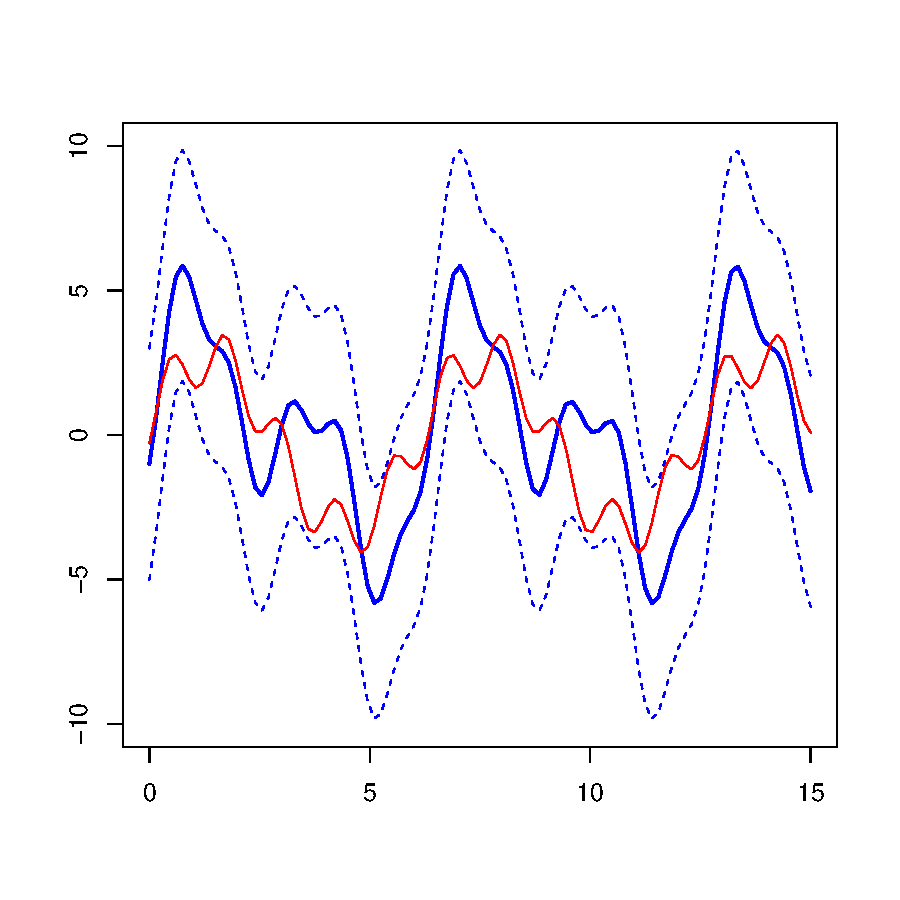
\includegraphics[width=0.7\textwidth]{tube.pdf}\end{center}
\end{frame}%}}}
\begin{frame}{Parasim Structure}%{{{
	\begin{itemize}
		\item core + extensions
		\item application combines the extensions
		\item own computational model
	\end{itemize}
\end{frame}%}}}
\begin{comment}
\begin{frame}{Parasim Lifecycle}%{{{
	\begin{center}
	\resizebox{.6\textwidth}{!}{
	\begin{tikzpicture}  	[node distance=.5cm,start chain=going below]
	\tikzset{>=stealth',
		event/.style={
			rectangle, 
			rounded corners, 
			fill=green!20,
			draw=black, very thick,
			text width=9em, 
			minimum height=3em, 
			text centered, 
			on chain},
	  	line/.style={draw, thick, <-},
		class/.style={
			rectangle, 
			rounded corners, 
			fill=black!10,
			draw=black, very thick,
			text width=8em, 
			minimum height=3em, 
			text centered,
			on chain},
		package/.style={
			rectangle,
			draw=black!50, dashed,
			rounded corners,
			inner sep=0.3cm,
			on chain},
	  	every join/.style={->, thick,shorten >=1pt}, 	
	 	scope/.style={decorate},
		code/.style={
			rectangle,
			draw=black!50, dashed,
			rounded corners,
			text width=15em,
			minimum height=3em, 
			text centered,
			node distance=7cm}
	}
		\node[event, join] (before-app-context) {BEFORE\\application context};
		\node[event, join] (processing) {PROCESSING};
		\node[code, left of=before-app-context] (code-create) {Manager m = Manager.create()};
		\node[package] (processing-package) {
			\begin{tikzpicture}
			\begin{scope}[solid, start branch=venstre, every join/.style={->, thick, shorten <=1pt}]
				\node[class] (enrichment) {enrichment};
				\node[class, on chain=going left] (configuration) {configuration};
				\node[class, on chain=going below] (lifecycle) {lifecycle};
				\node[class, on chain=going right] (extension-loader) {extension loading};
				\node[class, on chain=going right] (remote) {remote control};
				\node[class, on chain=going above] (logging) {logging};
			\end{scope}
			\end{tikzpicture}
		};
		\node[event, join] (started) {STARTED};
		\node[code, left of=started] (code-start) {m.start()};
		\node[package, join, inner sep=0.5cm, text width=15em, text centered] (other-extensions) {interaction with loaded extensions};
		\node[package, join, inner sep=0.5cm, text width=15em, text centered] (main-app) {main application code};
		\node[event, join] (stopping) {STOPPING};
		\node[event, join] (after-app-context) {AFTER\\application context};
		\node[code, left of=stopping] (code-shutdown) {m.destroy()};

		\begin{scope}[->, thick, shorten <=1pt] 
			\draw	(processing)	-> (processing-package);
		\end{scope}

		\begin{scope}[->, dashed, shorten <=1pt] 
			\draw	(code-create)	-> (before-app-context);
			\draw	(code-start)	-> (started);
			\draw	(code-shutdown)	-> (stopping);
		\end{scope}
	\end{tikzpicture}}
	\end{center}
\end{frame}%}}}
\begin{frame}{Computational Model}%{{{
	\lstinputlisting{ComputationImpl.java}
\end{frame}%}}}
\end{comment}
\begin{frame}%{{{
	\scream{DEMO}
\end{frame}%}}}
\begin{frame}{Number of Generated Trajectories}%{{{
	\begin{columns}[2]
		\begin{column}{0.5\textwidth}
			\begin{center}
				\textbf{Lorenz System}

				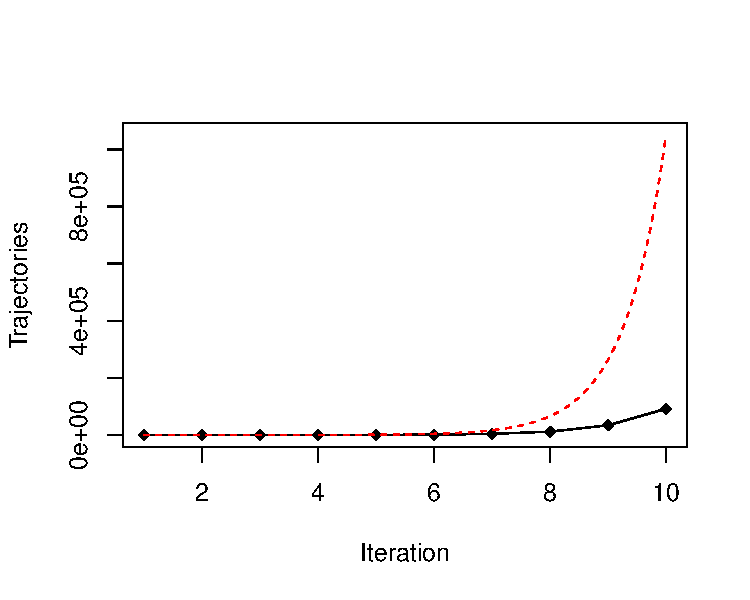
\includegraphics[width=\textwidth]{lorenz84-iterations-summary}
			\end{center}
		\end{column}
		\begin{column}{0.5\textwidth}
			\begin{center}
				\textbf{Lotka-Volterra}

				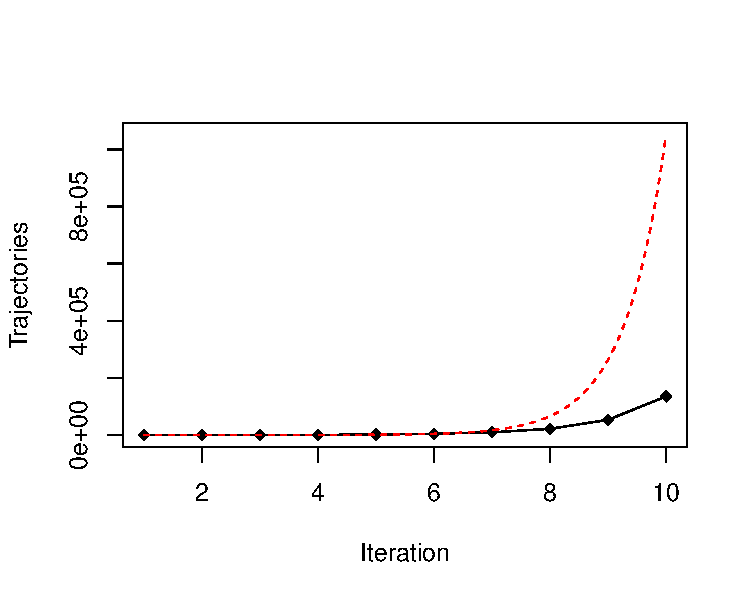
\includegraphics[width=\textwidth]{lotkav-iterations-summary}
			\end{center}
		\end{column}
	\end{columns}
\end{frame}%}}}
\begin{frame}{Scalability (Lorenz System)}%{{{
	\begin{columns}[2]
		\begin{column}{0.5\textwidth}
			\begin{center}
				\textbf{8 iterations,\\long property}

				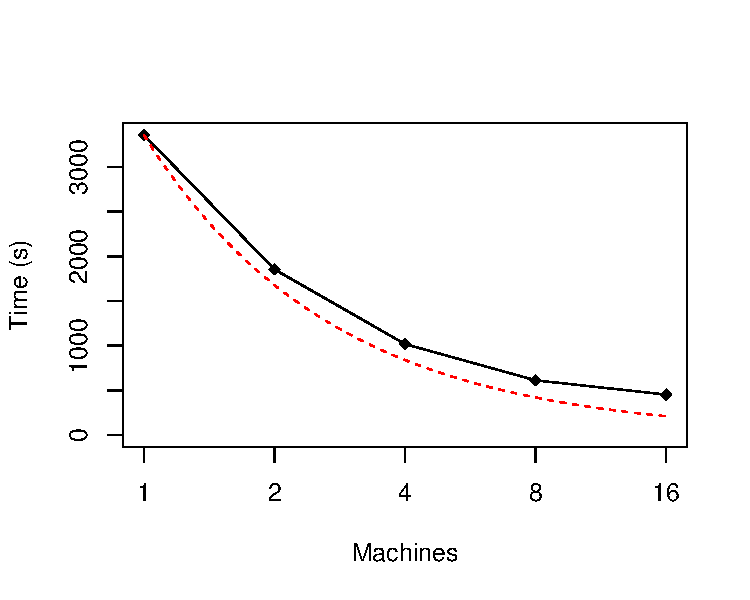
\includegraphics[width=\textwidth]{lorenz84-long-property-time}
			\end{center}
		\end{column}
		\begin{column}{0.5\textwidth}
			\begin{center}
				\textbf{10 iterations,\\short property}

				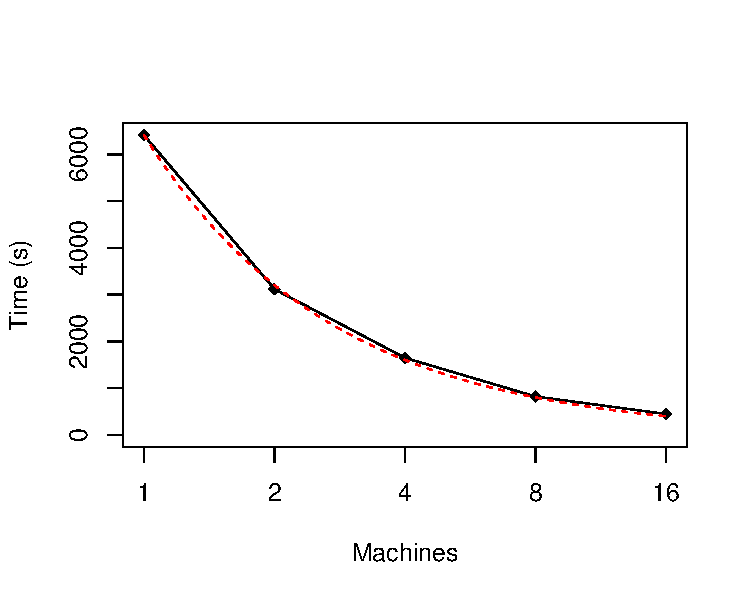
\includegraphics[width=\textwidth]{lorenz84-iterations-time}
			\end{center}
		\end{column}
	\end{columns}
\end{frame}%}}}
\end{document}
